\chapter{Shannonova kapacita}

\section{Formulace úlohy}

Představme si komunikační kanál, kterým posíláme zprávy. Tyto zprávy jsou složeny ze symbolů nějaké konečné abecedy. Vlivem šumu mohou být některé symboly druhou stranou špatně interpretovány a naším cílem je vybrat co největší množinu slov délky $k$ tak, aby žádná dvě odeslaná slova nebyla vlivem tohoto šumu zaměnitelná.

Problém si formalizujeme v řeči teorie grafů. Mějme neorientovaný graf $G = (V, E)$, kde množina vrcholů představuje symboly z konečné abecedy a dva vrcholy $x, y$ jsou spojeny hranou, pokud vrchol $x$ může být vlivem šumu zaměněn za $y$.

Maximální počet nezaměnitelných zpráv délky $1$ je roven $\alpha(G)$, kde $\alpha(G)$ značí velikost největší nezávislé množiny v grafu $G$. Pro popis delších zpráv definujeme \textbf{silný součin} $G \cdot H$ grafů $G$ a $H$ následovně
\begin{equation*}
    V(G \cdot H) = V(G) \times V(H),
\end{equation*}
\begin{equation*}
    \begin{split}
    E(G \cdot H) = &\left\{ (i,u)(j,v) \mid ij \in E(G) \wedge uv \in E(H) \right\} \cup \\
                   &\left\{ (i,u)(j,v) \mid ij \in E(G) \wedge u = v \right\} \cup \\
                   &\left\{ (i,u)(j,v) \mid i = j \wedge uv \in E(H) \right\}.
    \end{split}
\end{equation*}

\begin{pr}
Pro graf $P_4 = a-b-c-d-e$ je silný součin $P_4 \cdot P_4$ zobrazen na obrázku~\ref{fig:strong_product_P4_P4}, ze kterého je hezky vidět, že např. zpráva $cd$ (na obrázku červeně) může být zaměněna s $bc$, $bd$, $be$, $cc$, $ce$, $dc$, $dd$ a $de$ (na obrázku oranžově). Podobně pro další zprávy.
\end{pr}

\begin{figure}[h!]
    \centering
    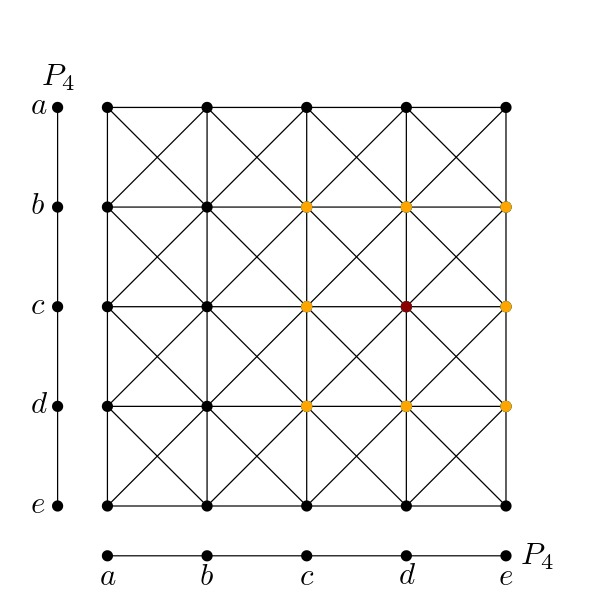
\includegraphics[width=0.5\textwidth]{img/strong_product_P4_P4.png}   
    \caption{$P_4 \cdot P_4$}
    \label{fig:strong_product_P4_P4}
\end{figure}

Pro jednoduchost budeme silný součin $k$ kopií grafu $G$ značit $G^k$. Tedy $\alpha(G^k)$ je maximální počet nezaměnitelných zpráv délky $k$. \textbf{Shannonova kapacita} grafu $G$ je definována jako
$$
    \Theta(G) = \sup \left\{ \alpha(G^k)^{1/k} \mid k = 1, 2, \dots \right\}.
$$

Neví se, zda pro libovolný graf $G$ existuje vůběc nějaký algoritmus, kterým bychom určili hodnotu $\Theta(G)$. Přesto je alespoň něco známo. Pro perfektní grafy Claude E. Shannon ukázal, že $\Theta(G) = \alpha(G)$. To také znamená, že pro perfektní grafy lze $\Theta(G)$ určit v polynomiálním čase. Dalším kdo se problémem zabýval byl László Lovász, který velmi hezkým způsobem ukázal, že kružnice délky $5$ má kapacitu $\sqrt{5}$. Na Lovászův postup se dále podíváme, protože vede k obecnému hornímu odhadu na $\Theta(G)$.

\section{$\Theta(C_5) = \sqrt{5}$}

Nejprve potřebujeme zavést několik pojmů. \textbf{Tenzorový součin} vektorů $u = \left(u_1, \dots, u_n \right)$ a $v = \left(v_1, \dots, v_m \right)$ je
$$
    u \circ v = \left( u_1 v_1, \dots, u_1 v_m, u_2 v_1, \dots, u_n v_m \right).
$$

Užitečné bude následující pozorování, které dává do souvislosti skalární a tenzorový součin.

\begin{pz}
    Nechť $x, u$ jsou vektory délky $n$ a $y, v$ jsou vektory délky $m$. Potom platí
    \begin{equation}
        \left( x \circ y \right)^T \left( u \circ v \right) = \left( x^T u \right) \left( y^T v \right).
        \label{eq:tensor_scalar_product}
    \end{equation}
\end{pz}

\begin{proof}
    Levá strana:
    \begin{equation*}
        \begin{split}
        & \left(x_1 y_1, x_1 y_2, \dots, x_1 y_m, \dots, x_n y_m \right)^T \left( u_1 v_1, u_1 v_2, \dots, u_1 v_m, \dots, u_n v_m \right) = \\
        & x_1 y_1 u_1 v_1 + x_1 y_2 u_1 v_2 + \dots + x_1 y_m u_1 v_m + \dots + x_m y_m u_n v_m
        \end{split}
    \end{equation*}
    Pravá strana:
    \begin{equation*}
        \begin{split}
            & \left( x_1 u_1 + \dots + x_n u_n \right) \cdot \left( y_1 v_1 + \dots + y_n v_m \right) = \\
            & x_1 y_1 u_1 v_1 + x_1 y_2 u_1 v_2 + \dots + x_1 y_m u_1 v_m + \dots + x_m y_m u_n v_m
        \end{split}
    \end{equation*}
\end{proof}

Mějme graf $G = (V,E)$, kde $V = \left\{ 1, \dots, n \right\}$. Systém $\left( v_1, \dots, v_n \right)$ jednotkových vektorů v Euklidovském prostoru takový, že
$$
    \forall ij \notin E \implies v_i \perp v_j
$$
nazýváme \textbf{ortonormální reprezentace} grafu $G$. Poznamenejme, že každý graf má nějakou ortonormální reprezentaci, např. $1 \mapsto e_1, \dots, n \mapsto e_n$.

\begin{lm}
    Nechť $\left( u_1, \dots, u_n \right)$ je ortonormální reprezentace grafu $G$ a $\left( v_1, \dots, v_m \right)$ je ortonormální reprezentace grafu $H$. Potom $u_i \circ v_j$ je ortonormální reprezentace grafu $G \cdot H$.
    \label{lemma:shannon}
\end{lm}

\begin{proof}
    Použijeme vztah \ref{eq:tensor_scalar_product}. $\left( u_i \circ v_j \right)^T \left( u_k \circ v_l \right) = \left( u_i^T u_k \right) \left( v_j^T v_l \right) = 0 \iff ik \notin E(G) \vee jl \notin E(H)$.
\end{proof}

\begin{figure}[h!]
    \centering
    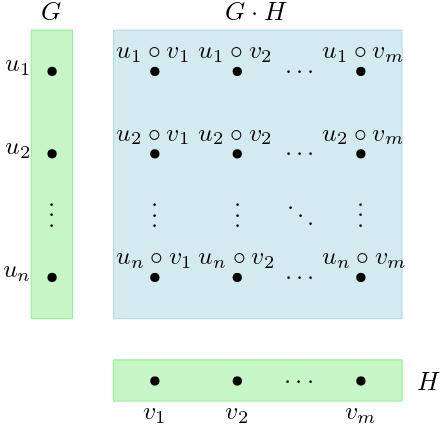
\includegraphics[width=0.5\textwidth]{img/shannon_lemma.png} 
    \caption{Lemma~\ref{lemma:shannon}}
\end{figure}

\noindent \textbf{Hodnotu} ortonormální reprezentace $\left(u_1, \dots, u_n \right)$ definujeme jako
$$
    \min_c \max_{i = 1, \dots, n} \frac{1}{\left( c^T u_i \right)^2}.
$$
Vektoru $c$, pro který nastává minimum říkáme \textbf{handle} dané ortonormální reprezentace.

Dále definujeme funkci $\vartheta(G)$ jako minimální hodnotu přes všechny ortonormální reprezentace grafu $G$. Ortonormální reprezentaci, pro kterou nastává minumum nazýváme \textbf{optimální}. Funkci $\vartheta(G)$ se říká \textbf{Lovászova theta funkce} a ona je právě již zmíněným horním odhadem na $\Theta(G)$. Podívejme se na některé její vlastnosti.

\begin{lm}
    $\vartheta(G \cdot H) \leq \vartheta(G) \vartheta(H)$
\end{lm}

\begin{proof}
    Nechť $\left( u_1, \dots, u_n \right)$ je optimální ortonormální reprezentace grafu $G$ s handle $c$ a $\left( v_1, \dots, v_m \right)$ je optimální ortonormální reprezentace grafu $H$ s handle $d$. Pak $c \circ d$ je jednotkový vektor a platí
    $$
        \vartheta(G \cdot H) \leq \max_{i,j} \frac{1}{\left( \left( c \circ d \right)^T \left( u_i \circ v_j \right) \right)^2} = \max_i \frac{1}{\left( c^T u_i \right)^2} \cdot \max_j \frac{1}{\left( d^T v_j \right)^2} = \vartheta(G)\vartheta(H).
    $$
\end{proof}

\begin{lm}
    $\alpha(G) \leq \vartheta(G)$
\end{lm}

\begin{proof}
    Mějme maximální nezávislou množinu $I \subseteq V(G)$ v grafu $G$ a optimální ortonormální reprezentaci $\mathcal{U} = \left( u_1, \dots, u_n \right)$ grafu $G$ s handle $c$. Platí
    $$
        \forall i,j \in I:\ i \neq j \implies u_i \bot u_j.
    $$
    Máme tedy systém ortonormálních vektorů $\left\{ u_i \in \mathcal{U} \mid i \in I \right\}$ v $\mathbb{R}^n$. Ten rozšíříme na ortonormální bázi $\mathcal{B}$. Potom $i$-tá souřadnice vektoru $c$ v bázi $\mathcal{B}$ je $c^T u_i$. Tedy
    $$
        1 = \| c \|^2 = \sum_{i=1}^n \left( c^T u_i \right)^2.
    $$
    Dále vynecháme přidáné vektory do ortonormální báze $\mathcal{B}$
    $$
        \sum_{i=1}^n \left( c^T u_i \right)^2 \geq \sum_{i \in I} \left( c^T u_i \right)^2.
    $$
    Poslední výraz přepíšeme
    $$
        \sum_{i \in I} \left( c^T u_i \right)^2 \geq |I| \cdot \min_{i \in I}\left( c^T u_i \right)^2 = \alpha(G) \cdot \min_{i \in I}\left( c^T u_i \right)^2.
    $$
    Předchozí výrazy dáme dohromady
    $$
        1 \geq \alpha(G) \cdot \min_{i \in I}\left( c^T u_i \right)^2,
    $$
    a dostáváme
    $$
        \alpha(G) \leq \frac{1}{\min_{i \in I}\left( c^T u_i \right)^2} = \max_{i \in I} \frac{1}{\left( c^T u_i \right)^2} \leq \max_{i \in V(G)} \frac{1}{\left( c^T u_i \right)^2} = \vartheta(G).
    $$
\end{proof}

\begin{lm}
    $\Theta(G) \leq \vartheta(G)$
\end{lm}

\begin{proof}
    Pro každé $k$ platí, že
    $$
        \alpha(G^k) \leq \vartheta(G^k) \leq \vartheta(G)^k.
    $$
    Odtud
    $$
        \sqrt[k]{\alpha(G^k)} \leq \vartheta(G),
    $$
    a limitním přechodem dostáváme požadovanou nerovnost
    $$
        \Theta(G) = \lim_{k \to \infty} \sqrt[k]{\alpha(G^k)} \leq \vartheta(G).
    $$
\end{proof}

\begin{vt}
    $\Theta(C_5) = \sqrt{5}$
\end{vt}

\begin{proof}
    Ukážeme konstrukci ortonormální reprezentace grafu $C_5$, ze které dostaneme horní odhad na $\Theta(C_5)$. Nechť $V(C_5) = \left\{ v_1, \dots, v_5 \right\}$ a $E(C_5) = \left\{ v_1v_2, v_2v_3, v_3v_4, v_4v_5, v_1v_5 \right\}$. Mějme vektory $\bar{u}_i$ ve tvaru
    $$
        \bar{u}_i = \left( \cos\frac{2 \pi i}{5}, \sin \frac{2 \pi i}{5}, z \right), i = 1, \dots, 5.
    $$
    Každý vektor $\bar{u}_i$ je svázán s vrcholem $v_i$. Chceme, aby dva vektory, které jsou příslušné nesousedním vrcholům, byly ortogonální. Tedy například $\langle \bar{u}_2, \bar{u}_5 \rangle = 0$. Dosadíme
    $$
        \left\langle \bar{u}_2, \bar{u}_5 \right\rangle = 
        \left\langle ( \cos\frac{4\pi}{5}, \sin\frac{4\pi}{5}, z ), \left( 1, 0, z \right) \right\rangle =
        \cos\frac{4\pi}{5} + z^2 = 0.
    $$
    Dostáváme tedy
    $$
        z = \sqrt{-\cos\frac{4\pi}{5}}.
    $$
    Definujeme ortonormální reprezentaci $\mathcal{U}$ grafu $C_5$ (projekce do první a druhé souřadnice, viz Obrázek~\ref{fig:umbrella_projection}) tak, že
    $$
        u_i = \frac{\bar{u}}{\| \bar{u} \|}, i = 1, \dots, 5,
    $$
    s handle $c = \left( 0, 0, 1 \right)$.
    Dostáváme
    $$
        \vartheta(C_5) \leq \vartheta(\mathcal{U}) = \max_{i = 1, \dots, 5} \frac{1}{(c^T u_i)^2} = \frac{1}{( c^T u_5)^2} = \frac{1 - \cos\frac{4\pi}{5}}{-\cos\frac{4\pi}{5}}.
    $$
    Do posledního výrazu dosadíme známou hodnotu pro $\cos 36^{\circ}$.
    $$
        \frac{1 - \cos\frac{4\pi}{5}}{-\cos\frac{4\pi}{5}} = \frac{1 + \frac{1 + \sqrt{5}}{4}}{\frac{1 + \sqrt{5}}{4}} = \frac{5 + \sqrt{5}}{1 + \sqrt{5}} = \sqrt{5}.
    $$
    Dostáváme
    $$
        \vartheta(C_5) \leq \sqrt{5}.
    $$
    Této ortonormální reprezentaci se říká \textbf{Lovászův deštník}, viz Obrázek~\ref{fig:umbrella}. Druhou nerovnost $\vartheta(C_5) \geq \sqrt{5}$ dostaneme snadno. Sice $\alpha(C_5) = 2$, ale $\alpha(C_5^2) = 5$. Z čehož plyne druhá nerovnost.
\end{proof}

\begin{figure}[h!]
    \centering
    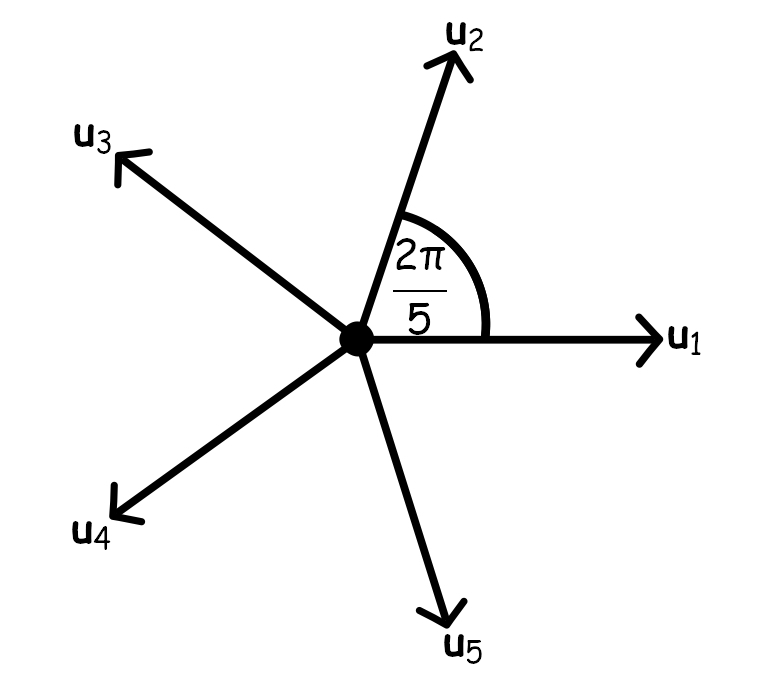
\includegraphics[width=0.5\textwidth]{img/umbrella_projection.png} 
    \caption{Projekce $u_i$ do první a druhé souřadnice.}
    \label{fig:umbrella_projection}
\end{figure}

\begin{figure}[h!]
    \centering
    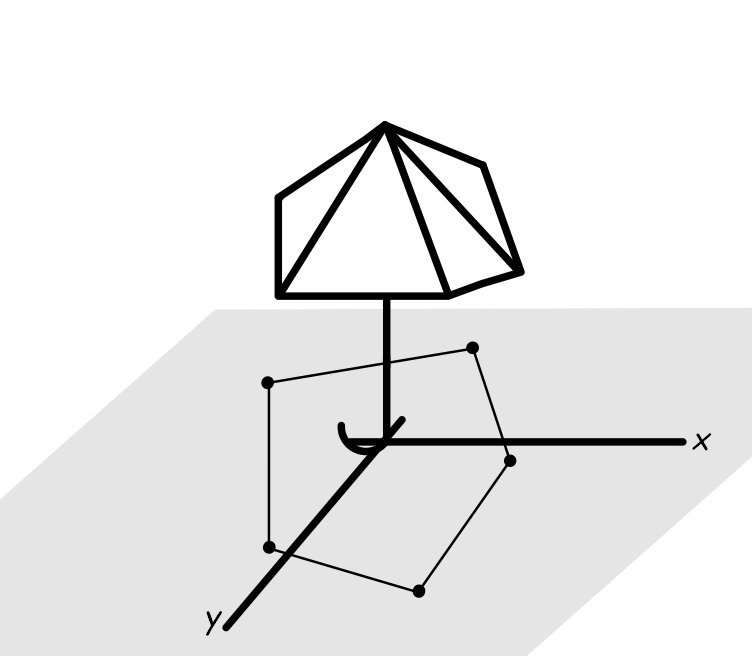
\includegraphics[width=0.5\textwidth]{img/umbrella.png} 
    \caption{Lovászův deštník.}
    \label{fig:umbrella}
\end{figure}


\section{Semidefinitní programy pro $\vartheta(G)$}

\subsection*{Program pro $1/\sqrt{\vartheta}$}

První formulací je semidefinitní program, jehož řešením je hodnota $\frac{1}{\sqrt{\vartheta}}$. Mějme graf $G = (V,E)$. Hodnota $\vartheta(G)$ je z definice
$$
    \vartheta(G) = \min_\mathcal{U} \vartheta(\mathcal{U}) = \min_\mathcal{U} \min_{\|c\|=1} \max_{i \in V(G)} \frac{1}{\left( c^T u_i \right)^2},
$$
kde $\mathcal{U}$ probíhá přes všechny ortonormální reprezentace grafu $G$. Pokud se stane, že $c^T u_i \leq 0$, potom místo $u_i$ budeme dále uvažovat vektor $-u_i$. Můžeme tedy předpokládat, že $\forall i \in V(G):\ c^T u_i \geq 0$. Potom hodnotu $1/\sqrt{\vartheta(G)}$ můžeme vyjádřit jako
$$
    \frac{1}{\sqrt{\vartheta(G)}} = \max_\mathcal{U} \frac{1}{\sqrt{\vartheta(\mathcal{U})}} = \max_\mathcal{U} \max_{\|c\|=1} \min_{i \in V(G)} c^T u_i.
$$
Z čehož dostaneme následující vektorový program
\begin{equation}\tag{VP1}
    \begin{split}
        &\max t \\
        &\forall ij \in E(\bar{G}):\ \langle u_i, u_j \rangle = 0 \\
        &\forall i \in V(G):\ \langle c, u_i \rangle \geq t \\
        &\forall i \in V(G):\ \| u_i \| = 1 \\
        &\| c \| = 1.
    \end{split}
    \label{eq:VP1}
\end{equation}

Z vektorového programu~\ref{eq:VP1} dále odvodíme semidefinitní program. Budeme uvažovat matici
$$
    X =
    \begin{bmatrix}
        \horzbar & c^T    & \horzbar \\
        \horzbar & u_1^T  & \horzbar \\
                 & \vdots &          \\
        \horzbar & u_n^T  & \horzbar
    \end{bmatrix}
    \begin{bmatrix}
        \vertbar & \vertbar &       & \vertbar \\
        c        & u_1      & \dots & u_n      \\
        \vertbar & \vertbar &       & \vertbar \\
    \end{bmatrix},
$$
která je samozřejme pozitivně semidefinitní.
Podmínkám $\forall i \in V(G):\ \| u_i \| = 1$ a $\|c\|=1$ odpovídá podmínka $x_{ii} = 1$ pro $i = 0, 1, \dots, n$ (pro teď budeme indexovat matici $X$ od $0$). Podmínku $\forall ij \in E(\bar{G}):\ \langle u_i, u_j \rangle = 0$ přepíšeme na
$$
    \forall ij \in E(\bar{G}):\ x_{ij} = 0.
$$
A konečně poslední podmínku $\forall i \in V(G):\ \langle c, u_i \rangle \geq t$ přepíšeme takto
$$
    \forall i \in V(G):\ x_{0i} \geq t.
$$
Dostáváme tedy semidefinitní program
\begin{equation}\tag{SDP1}
    \begin{split}
        &\max t \\
        &x_{ii} = 1, i = 0, 1, \dots, n \\
        &\forall ij \in E(\bar{G}):\ x_{ij} = 0 \\
        &\forall i \in V(G):\ x_{0i}  \geq t \\
        &X \succeq 0.
    \end{split}
    \label{eq:SDP1}
\end{equation}


\subsection*{Program pro $\vartheta$}

V původním článku od L.~Lovásze \textbf{[REF]} je další semidefinitní program, jehož řešením je přímo hodnota $\vartheta(G)$.

\begin{equation}\tag{SDP2}
    \begin{split}
        &\max \langle X, J \rangle \\
        &\forall ij \in E(G):\ x_{ij} = 0 \\
        &\textbf{Tr}\ X = 1 \\
        &X \succeq 0,
    \end{split}
    \label{eq:SDP2}
\end{equation}
kde $J$ je matice samých jedniček.

\section{$\vartheta$ a související grafové parametry}

Začneme tzv. Sendvičovou větou a dále zaměříme na grafy $C_5$, $C_7$, Petersenův graf, $K_5$ a $S_5$.

\begin{vt}\textbf{[REF]}
    Mějme graf $G$ a jeho doplněk $\bar{G}$. Potom
    $$
        \alpha(G) \leq \vartheta(G) \leq \chi(\bar{G}).
    $$
\end{vt}

\subsection*{$\alpha(G)$ pro vybrané grafy}
Je zřejmé, že pro $\alpha(C_5) = 2$, $\alpha(C_7) = 3$, $\alpha(K_5) = 1$ a $\alpha(S_5) = 5$. Na obrázku~\ref{fig:alpha_petersen} je, pro Petersenův graf, nezávislá množina velikosti $4$. Probírkou všech možností zjistíme, že větší nezávislou množinu se nám najít nepodaří.

\begin{figure}[h!]
    \centering
    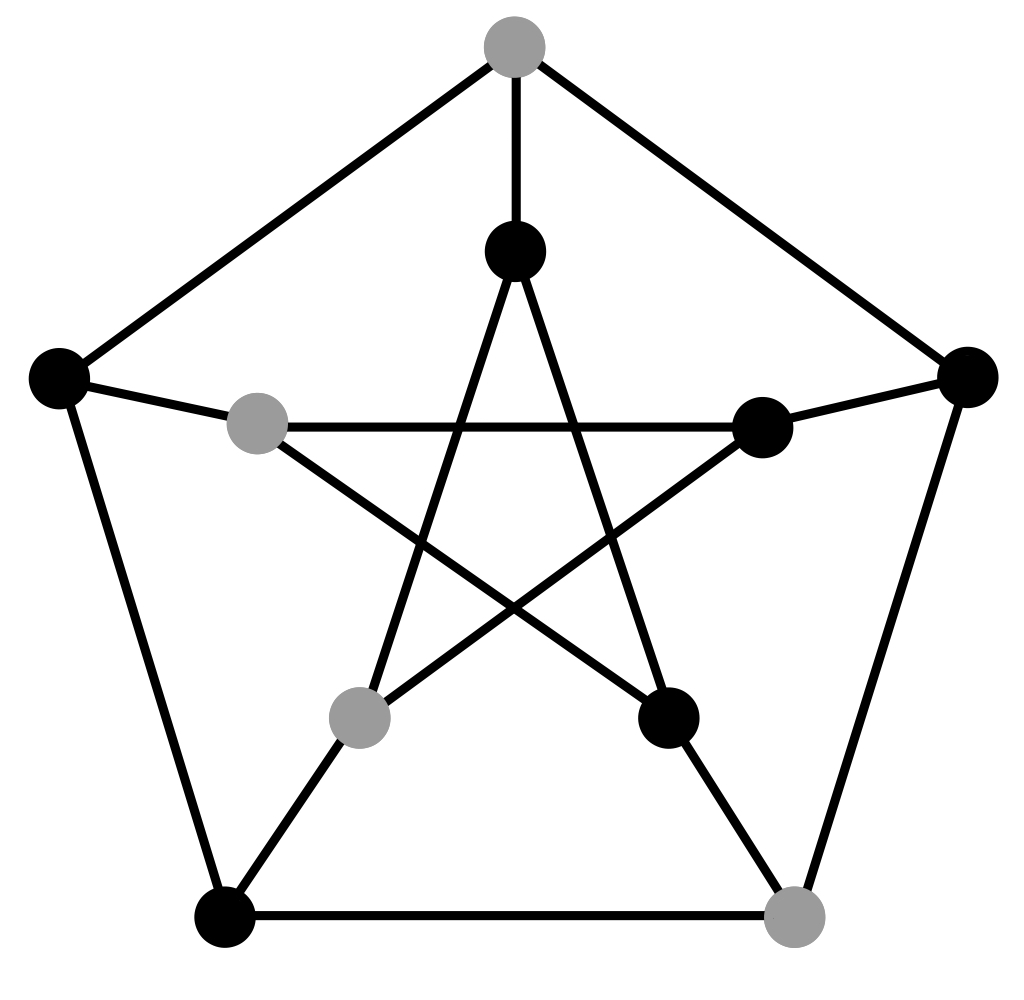
\includegraphics[width=0.5\textwidth]{img/alpha_petersen.jpeg}   
    \caption{Největší nezávislá množina v $GP_{5,2}$.}
    \label{fig:alpha_petersen}
\end{figure}

\subsection*{$\chi(\bar{G})$ pro vybrané grafy}

Doplněk $C_5$ je opět $C_5$ a lichá kružnice má chromatické číslo $3$. $K_5$ má jako svůj doplněk diskrétní graf, který má chromatické číslo $1$. U hvězdy $S_5$ dostaneme jako doplněk graf s šesti vrcholy, kde pět z nich tvoří úplný graf a jeden vrchol nemá žádného souseda. Takový graf má chromatické číslo $5$. Pro Petersenův graf je jeho doplněk $T_5$, který má $\chi(T_5) = 5$ ($T_5$ viz Obrázek~\ref{fig:complement_petersen}). Nakonec doplněk k $C_7$ je na obrázku~\ref{fig:complement_c7} a opět probírkou všech možností zjistíme, že chromatické číslo je $4$.

\begin{figure}[h!]
    \centering
    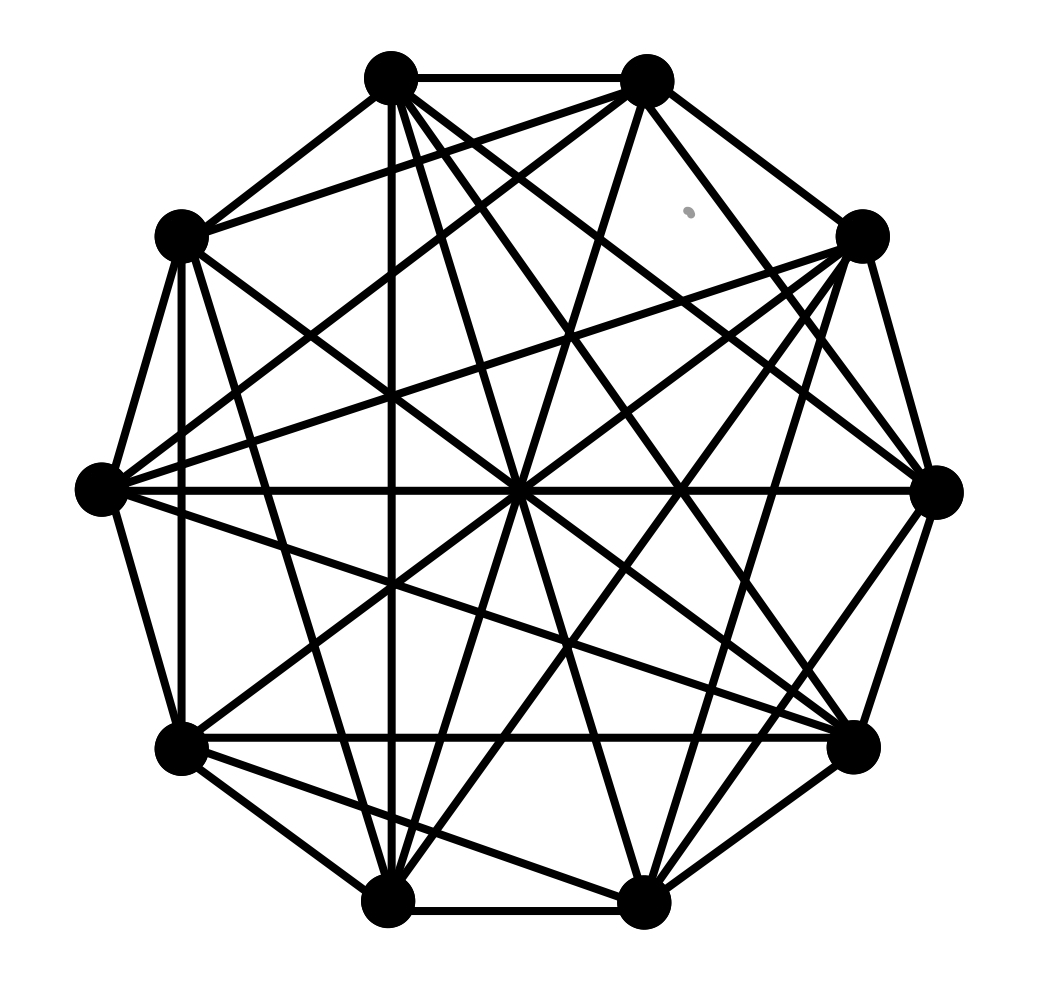
\includegraphics[width=0.5\textwidth]{img/complement_petersen.jpeg}   
    \caption{Triangular graf $T_5$.}
    \label{fig:complement_petersen}
\end{figure}

\begin{figure}[h!]
    \centering
    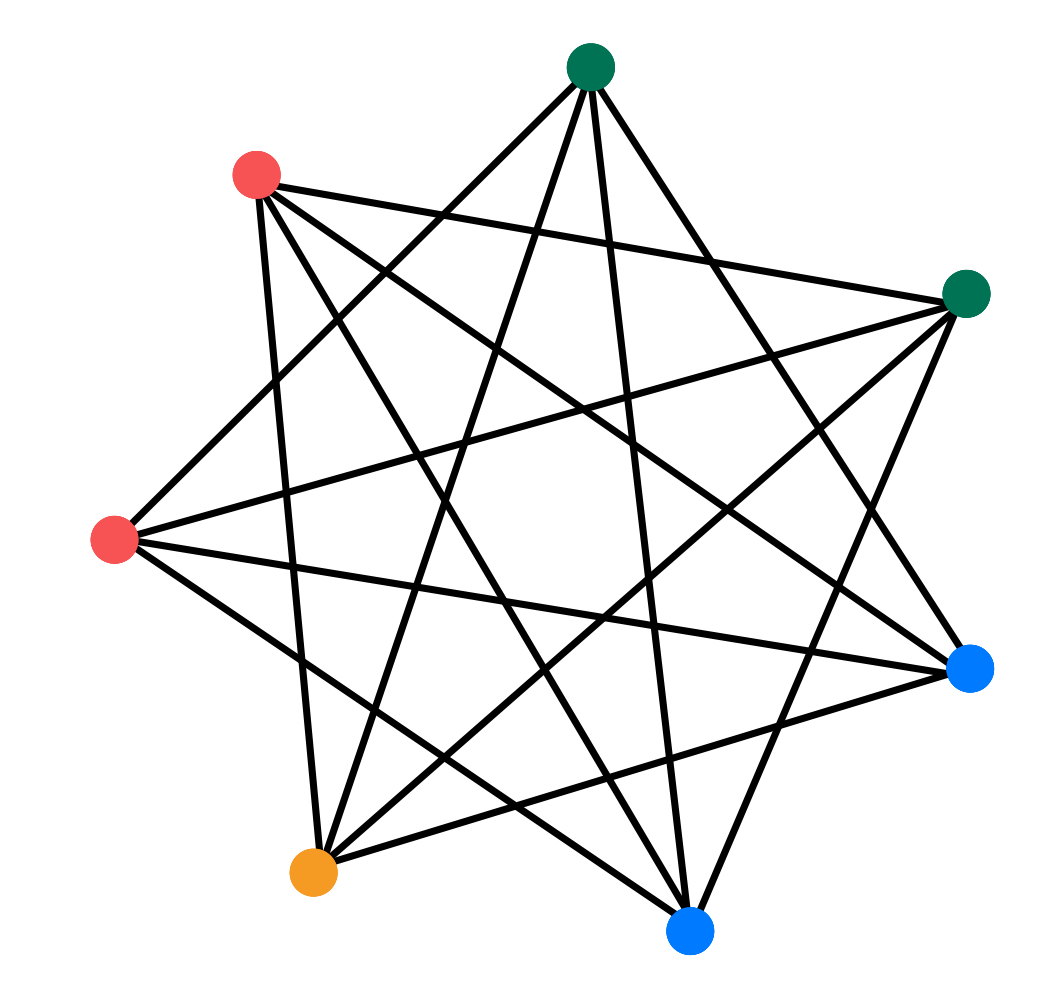
\includegraphics[width=0.5\textwidth]{img/complement_c7.jpeg}   
    \caption{Obarvení $\bar{C_7}$.}
    \label{fig:complement_c7}
\end{figure}

\subsection*{$\vartheta(G)$ pro vybrané grafy}

Dříve jsme ukázali, že $\vartheta(C_5) = \sqrt{5} \approx 2.2361$. Navíc pro liché $n$ \textbf{[REF]} platí, že
$$
    \vartheta(C_n) = \frac{n \cdot \cos(\frac{\pi}{n})}{1 + \cos(\frac{\pi}{n})}.
$$
Dostáváme tedy, že $\vartheta({C_7}) \approx 3.3177$. Zbylé hodnoty plynou ze sendivičové věty. V tabulce~\ref{tab:sandwitch} jsou shrnuty všechny zmíněné hodnoty.

\begin{table}[h!]
    \centering
    \begin{tabular}{ c | c c c }
        $G$        & $\alpha(G)$ & $\vartheta(G)$ & $\chi(\bar{G})$ \\
        \hline
        $C_5$      & $2$         & $2.2361$       & $3$ \\  
        $C_7$      & $3$         & $3.3177$       & $4$ \\
        $GP_{5,2}$ & $4$         & $4$            & $5$ \\
        $K_5$      & $1$         & $1$            & $1$ \\
        $S_5$      & $5$         & $5$            & $5$
    \end{tabular}
    \caption{$\alpha(G)$, $\vartheta(G)$, $\chi(\bar{G})$ pro vybrané grafy.}
    \label{tab:sandwitch}
\end{table}

\subsection*{Co víme o $\Theta(G)$}

Shannonova kapacita je známá jen pro několik málo grafů. V \textbf{[REF]} Shannon dal dolní odhad na $\Theta(C_5)$ a až za 23 let Lovász ukázal pomocí konstrukce, kterou jsme si ukázali výše, že $\Theta(C_5) = \sqrt{5}$. Ve stejném článku \textbf{[REF]} je důkaz, že kapacita Petersenova grafu $GP_{5,2}$ je $4$. Triviální případy $S_5$ a $K_5$ dostaneme ze sendvičové věty, tj. $\Theta(S_5) = 5$ a $\Theta(K_5) = 1$. Naopak pro $C_7$ hodnotu $\Theta$ neznáme. Máme dolní odhad $\alpha(C_7) = 3$ a horní odhad $\vartheta(C_7) \approx 3.3177$. Lepší dolní odhad, než dává $\alpha(C_7)$, ukázali Polak a Schriever \textbf{[REF]} tak, že pomocí počítače našli nezávislou množinu v grafu $C_7^5$ velikosti $367$. Z čehož dostaneme dolní odhad $\sqrt[5]{367} \approx 3.2579$. Hodnota $\Theta(C_7)$ je tedy někde mezi
$$
    3.2578 < \Theta(C_7) \leq 3.3177.
$$

Poznamenejme, že vylepšit dolní odhad na $\Theta(C_7)$ je výpočetně náročná úloha. Už pro $C_7^4$ se pomocí formulace
\begin{equation*}
    \begin{split}
        &\max \sum_{i=1}^n x_i \\
        &\forall ij \in E:\ x_i + x_j \leq 1 \\
        &\forall i \in V:\ x_i \in \left\{ 0, 1 \right\}
    \end{split}
\end{equation*}
nenajde užitečná nezávislá množina, která by měla velikost alespoň $108$ \textbf{[REF-Vesel-Žertovnik]}. K výpočtu byl použit framework \textbf{Gurobi} a program po $7$ měsících našel pouze nezávislou množinu velikosti $102$, která dává dolní odhad $\sqrt[4]{102} \approx 3.1779$.


\section{Experimenty}

Porovnáme formulace \ref{eq:SDP1} a \ref{eq:SDP2}, které byly naimplementovány ve frameworku \textbf{Mosek}, na lichých kružnicích s přesnou hodnotou a dále určíme hodnoty $\vartheta$ pro náhodné grafy řádu $30$.

\begin{center}
    \begin{tabular}{ c | c c c }
    $n$    & $\vartheta(C_n)$ & \ref{eq:SDP1} & \ref{eq:SDP2} \\
    \hline
    $5$    & $X$              & $X$           & $X$           \\
    $7$    & $X$              & $X$           & $X$           \\
    $9$    & $X$              & $X$           & $X$           \\
    $11$   & $X$              & $X$           & $X$           \\
    $13$   & $X$              & $X$           & $X$           \\
    $15$   & $X$              & $X$           & $X$           \\
    \end{tabular}
\end{center}

\begin{center}
    \begin{tabular}{ c c c c c c c c c c c c }
    $m$    & \ref{eq:SDP1} & \ref{eq:SDP2} \\
    \hline
    $0$    & $X$           & $X$           \\
    $43$   & $X$           & $X$           \\
    $87$   & $X$           & $X$           \\
    $130$  & $X$           & $X$           \\
    $174$  & $X$           & $X$           \\
    $217$  & $X$           & $X$           \\
    $261$  & $X$           & $X$           \\
    $304$  & $X$           & $X$           \\
    $348$  & $X$           & $X$           \\
    $391$  & $X$           & $X$           \\
    $435$  & $X$           & $X$           \\
    \end{tabular}
\end{center}


